\chapter{Speech Processing}\label{ch:speech_processing}

Speech is an effortless and highly efficient form of communication.
Continuous speech recognition software is readily available from stores and it allows the user to interact with its surrounding without the need of written commands
\cite[p.~396]{callan2003artificial}. Amazon`s Alexa 
\cite{Alexa} and Microsoft`s Cortana 
\cite{Cortana} are perfect examples of home companions that are able to perform basic tasks received via voice commands.
As speech recognition increases in accuracy to the high nineties, reaching a performance of 99\% means that this technology will make the leap from being annoying to use to becoming the main way we interact with computers. 
This idea is further backed up by the fact that people tend to speak much faster than they are able to type \cite{Speed}.
In some cases, speech can be three times faster in conveying information than typing and for professional debaters,
speaking can be even six times faster. \\

Words are carried as sound waves, which are analog signals.
In order for the speech to be processed,
it needs to be run through a signal processor that selects the frequencies and amplitude of the signal.
Further on, the signal is mapped to individual sound units called phones.
These phones need to be identified and grouped in such a way to ensure that each word has a different phonetic structure,
otherwise, words would be impossible to distinguish from one another. \\

\begin{table}[]
\centering
\caption{Phones}
\label{my-label}
\begin{tabular}{ll}
{[}ay{]} & \underline{ir}is \\
{[}b{]}  & \underline{b}in  \\
{[}er{]} & \underline{bir}d \\
{[}l{]}  & \underline{l}ip  \\
{[}p{]}  & \underline{p}in  \\
{[}th{]} & \underline{thi}n
\end{tabular}
\end{table}

Phones can have different sounds depending on the context. 
For example, the phone th in the word \textit{three} has a different sound to th in \textit{then}. 
To overcome these different variations of the same phones, 
it is better to abstract the phones into a generalized grouping called a \textbf{phoneme}.
Phonemes are written in-between forward slashes
(\textit{/th/}) and they will have a specific pronunciation for each sound, depending on the context.
These phonemes are used as a transitional layer when trying to convert speech to text and vice versa,
when speech needs to be synthesized.\\

\section{Signal processing}

Sound waves that carry human speech are variations in air pressure.
The key components of a sound wave are its \textbf{amplitude},
which measure the intensity of the sound and the \textbf{frequency}, which describes the rate at which the amplitude varies over time.
When speaking in a microphone,
the change in air pressure causes the diaphragm to oscillate.
The size of the oscillations is directly proportional to the amplitude of the signal,
while the rate at which the diaphragm oscillates gives represents the rate at which the air pressure changes.
At specific time intervals,
the signal can be sampled and the data can be used in a wide array of digital signal processing tools.
For example, the digital signal can be plotted as an x-y plot,
where the y-axis defines the amplitude and the x-axis shows the time.
The frequency can be easily be determined from the plot as we find the number of cycles that the signal does per second.\\

Although a visual difference can be seen when plotting vowels and consonants,
a visual inspection of the waveform will not reveal any critical information, making it impossible to see all the phonemes.\\

To feed this information to the neural network, some preprocessing and signal manipulation is required so the input can be understood and passed through the neurons.
These steps are expanded upon in the following subsections.

\subsubsection{ Preprocessing}

No matter how powerful and how advanced a computer is,
it still works in discrete time.
In order to represent an analogue signal on the computer we have to sample it according to the Nyquist–Shannon sampling theorem,
which states that the sampling frequency has to be at least double the frequency of the original signal in order to replicate the original signal without aliasing.
For a better understanding of the process, a visual representation of the word "Hello" as it is formed for the input of the neural network is shown in figure\ref{fig:Waveform} where it is sampled at 8000 Hz.

%\begin{figure}[h!]
%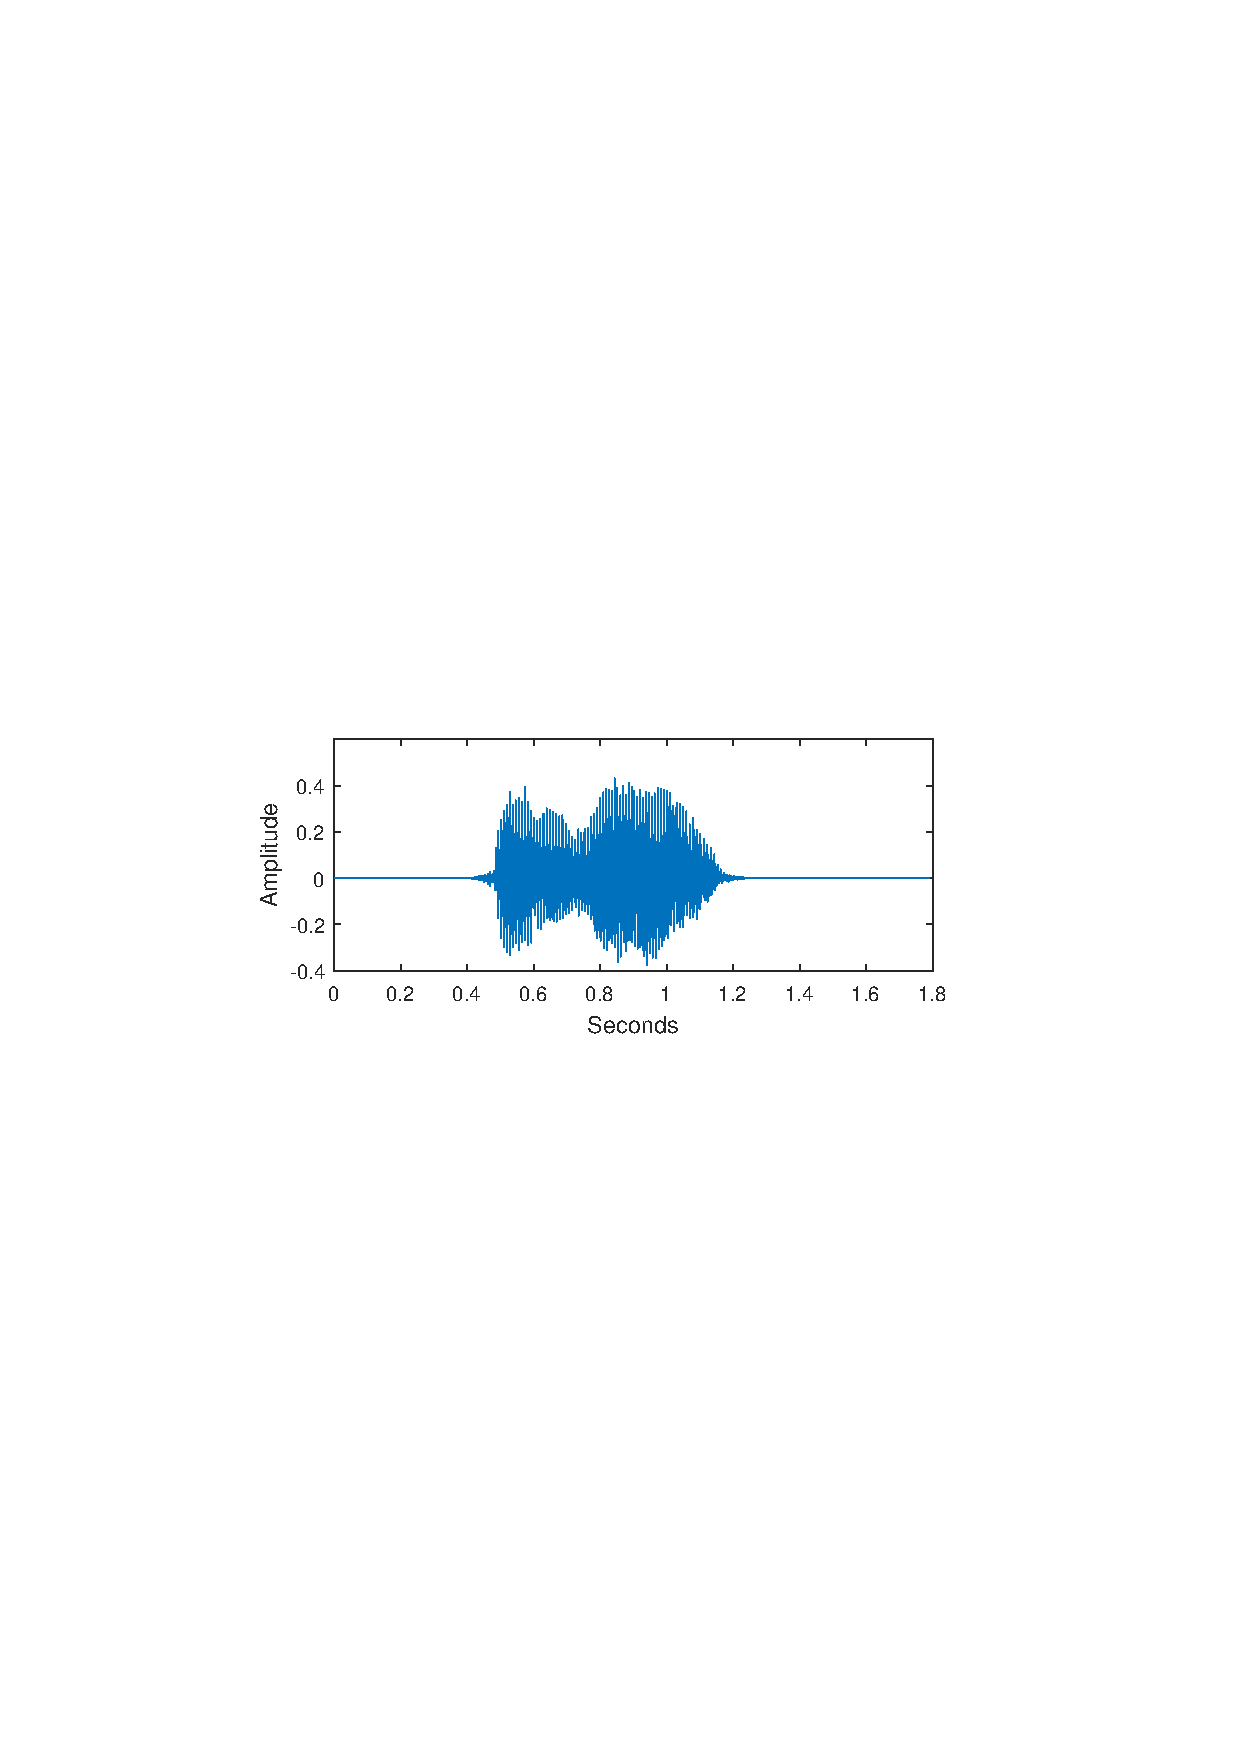
\includegraphics[trim={35 15 15 15},clip]{Hello_waveform}
%\centering
%\caption{Waveform for the word: "Hello"}
%\label{fig:Waveform}
%\end{figure}

\subsubsection{ Fourier transform}

To analyse a discrete signal we use the Fourier transform. 
This allows us to convert the signal in the frequency domain and deconstruct it in a series of simple sine waves. 
These sine waves have specific amplitudes and frequencies and while plotting the FFT of the signal, 
the dominant waves can be identified by the intensity of the amplitude.\\

In Figure \ref{fig:FFT}, a visual representation of the FFT is shown. 
It can be seen that there are a lot of frequencies that make up the word "Hello". 
The dominant ones are in the range of 500Hz. 
Considering that this recording has a minimum amount of noise,
we have to consider the full range of the frequencies,
from zero and up to 3500Hz.


%\begin{figure}[h]
%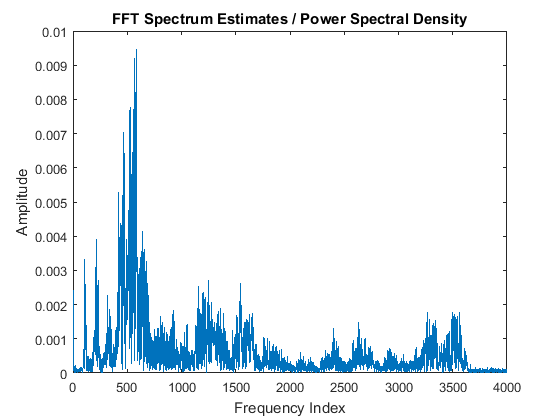
\includegraphics[trim={15 4 7 7},clip]{FFTpicture2}
%\centering
%\caption{Example of the FFT function computed for the word "Hello"}
%\label{fig:FFT}
%\end{figure}

\subsubsection{ Spectrogram}

The spectrogram of the signal was computed from the FFT and it shows a visual representation of the spectrum of frequencies marked by the intensity of the color. After the spectrogram is sliced into 25 ms chunks, it is feed as the input to the network. A neural network can find patterns in this data more easily than raw sound waves because audio data and patterns can be seen in the graph.

\begin{figure}[!htb]
    \centering
    \begin{minipage}{0.5\textwidth}
        \centering
        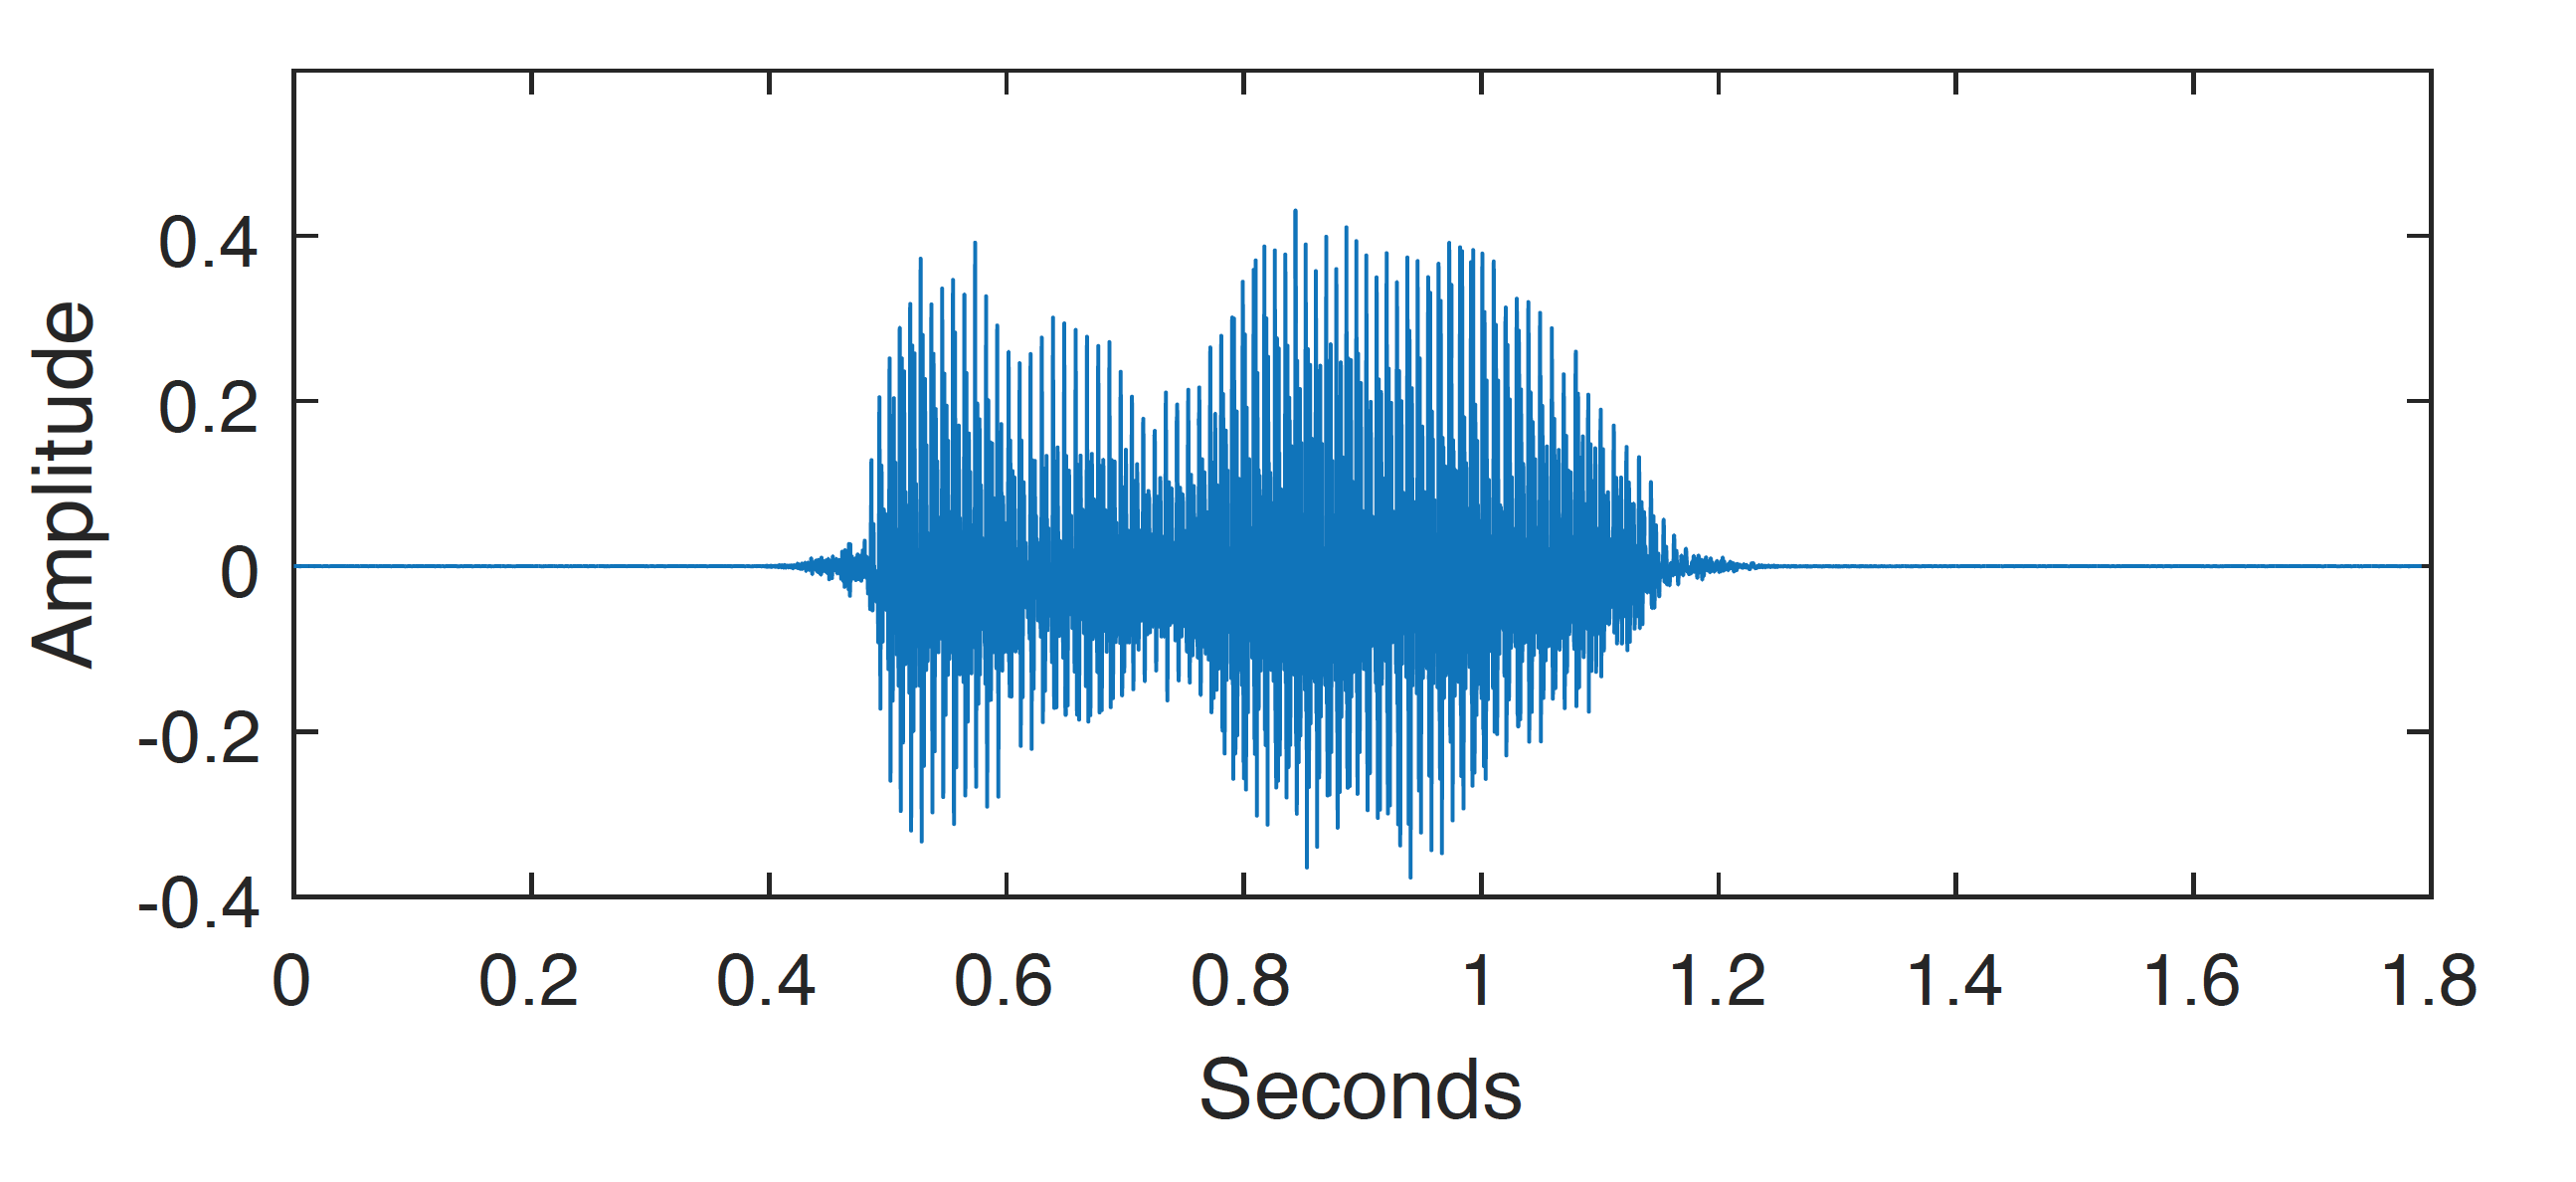
\includegraphics[width=\textwidth,
        height=0.2\textheight]
        {speech_processing/00_Hello_waveform}
        \caption{Left caption.}
        \label{fig:prob1_6_2}
    \end{minipage}%
    \begin{minipage}{0.5\textwidth}
        \centering
        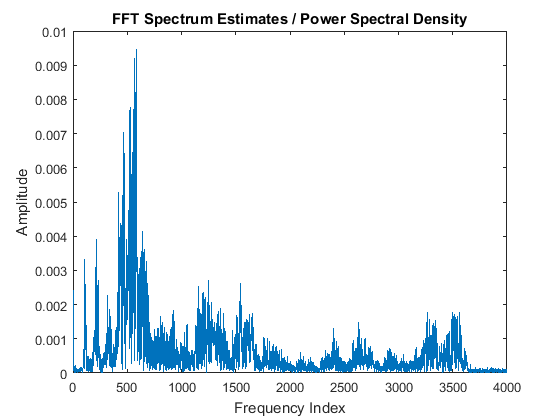
\includegraphics[width=\textwidth,
        height=0.2\textheight]
        {speech_processing/01_FFT_Of_Hello}
        \caption{Right caption.}
        \label{fig:prob1_6_1}
    \end{minipage}
\end{figure}

\todo{The figures are on GitHub, need to figure out how they work in LaTeX}